次に,画像認識分野におけるCNNについて説明する.
画像認識分野における課題は,画像中に存在する物体の種類を正確に認識することであり,特に畳み込みニューラルネットワークによる活躍が目覚ましい分野の一つである.
畳み込みニューラルネットワークを用いた手法では,画像を入力とし,多層の畳み込み層を経て特徴量を抽出し,最終的に全結合層を用いて出力を画像に存在する物体の種類(クラス)とするものが多い(\ref{fig:classification}).
\begin{figure}[ht]
  \centering
  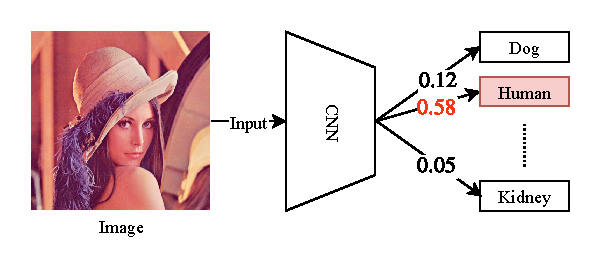
\includegraphics[width=14cm]{8_appendix/img/image_classification.pdf}
  \caption{Classification with CNN.}
  \label{fig:classification}
\end{figure}

本研究において用いるモデルの多くがこれらのモデルに基づいている,
ここでは,その中でも代表的なモデルについて説明する.
\subsubsection{LeNet-5}
    LeNet-5\cite{lecun1998gradient, lecun1999object}は畳み込みニューラルネットワークが注目を集める以前に提案されていた手法であり,6層構造のCNNである.
    LeNetの構造を図\ref{fig:lenet}に示す.
    このモデルは32$\times$32ピクセルのパッチ画像の入力を想定している.
    LeNetで利用されている畳み込み層の基本的な考え方は1989年ごろから提案されていた\cite{lecun1989backpropagation}.
    \begin{figure}[ht]
      \centering
      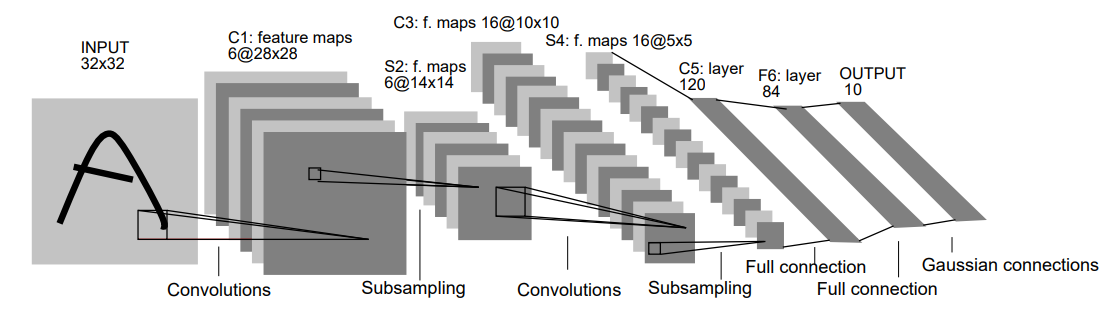
\includegraphics[width=14cm]{8_appendix/img/lenet.png}
      \caption{Architecture of LeNet \cite{lecun1998gradient}.}
      \label{fig:lenet}
    \end{figure}

\subsubsection{AlexNet}
    畳み込みニューラルネットワーク自体は前述のLeNetにて提案されていたが,それが大きく注目されるのは2012年,ImageNet Large Scale Visual Recognition Challenge(ILSVRC)\cite{ILSVRC15}にて,AlexNet\cite{krizhevsky2012imagenet}が画像認識分野において最も優れた成績を示してからである.
    図\ref{fig:alexnet}にネットワーク構造の概要図を示した.
    このモデルは5層の畳み込み層と3層の全結合層で構成され,パラメータ数は約6000万である.
    \begin{figure}[ht]
      \centering
      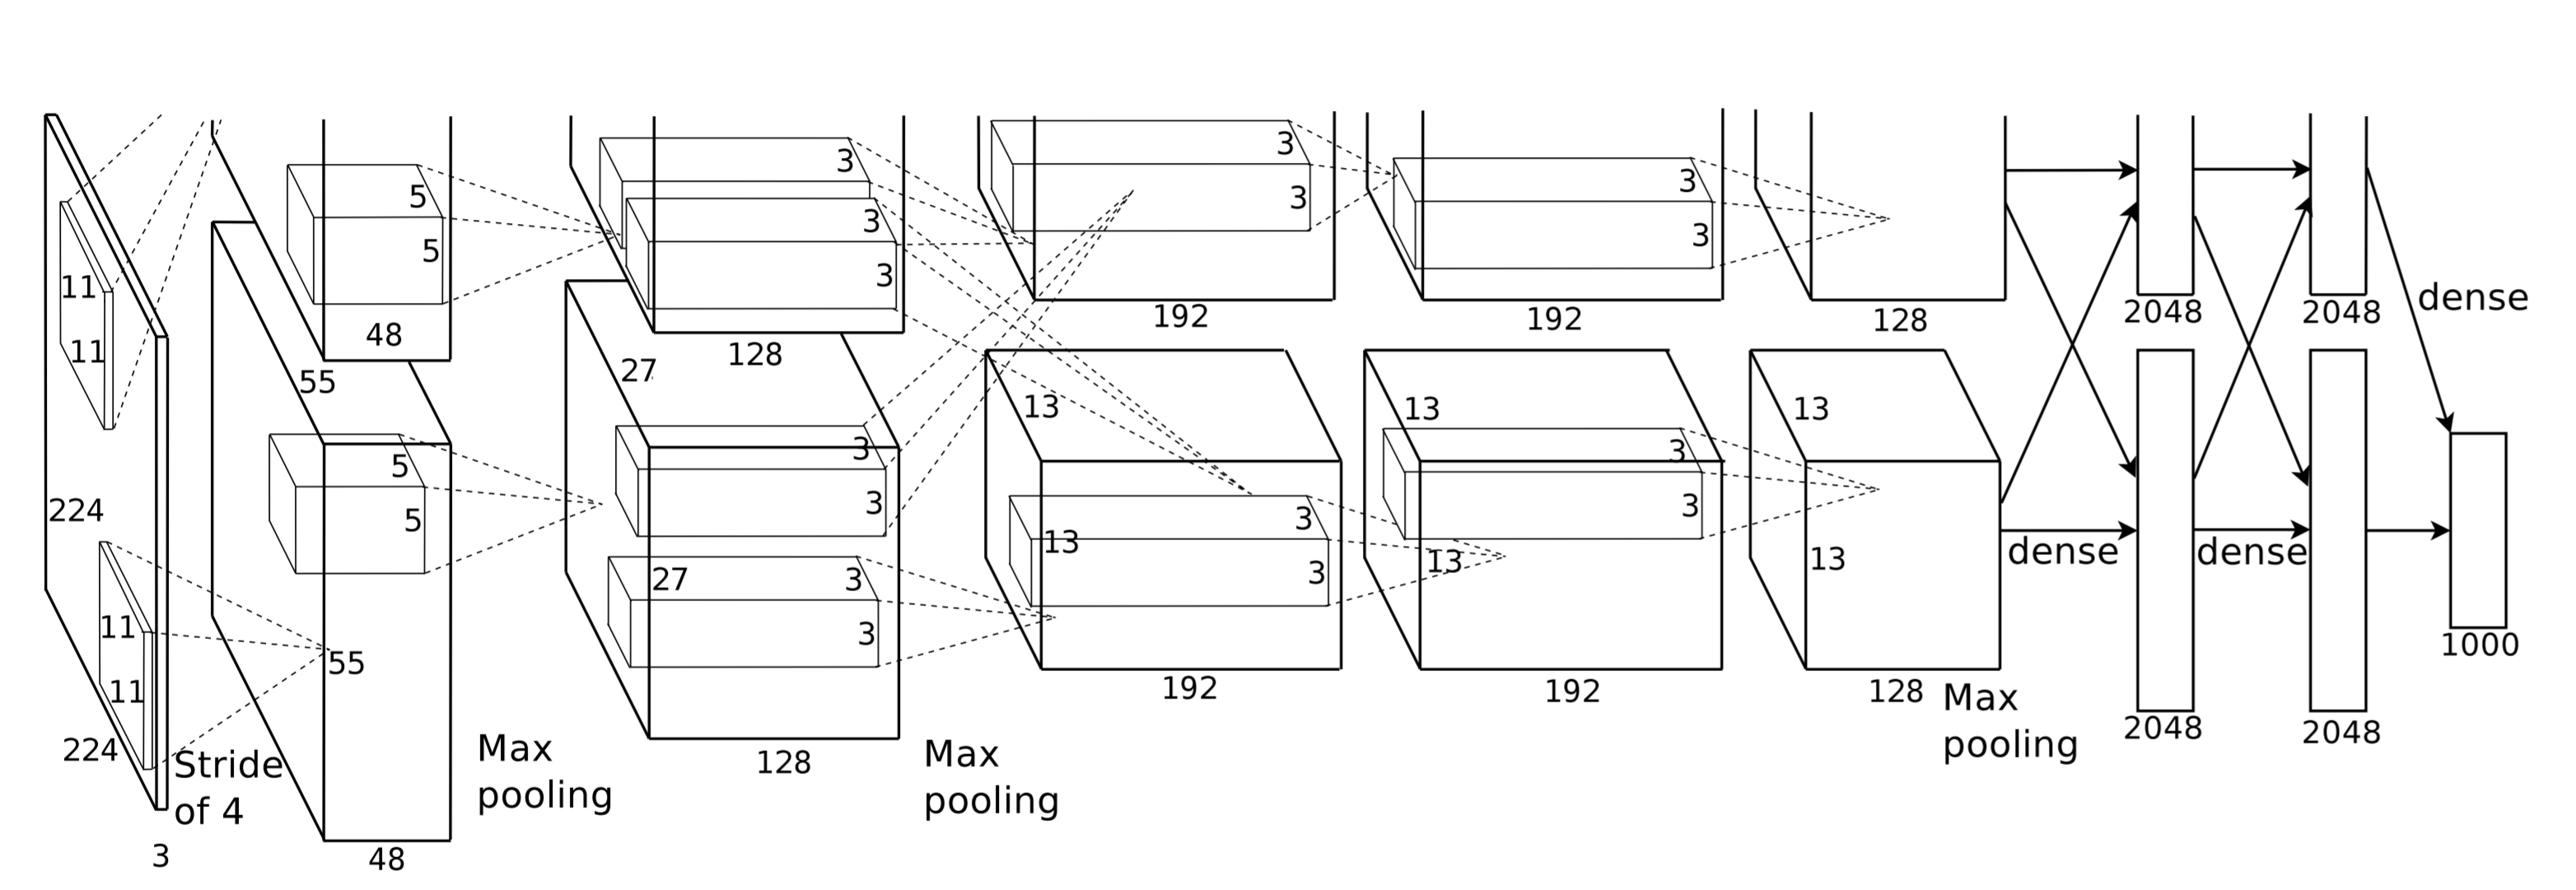
\includegraphics[width=14cm]{8_appendix/img/alexnet.png}
      \caption{Architecture of AlexNet \cite{krizhevsky2012imagenet}.}
      \label{fig:alexnet}
    \end{figure}
    AlexNetはLeNetと異なり,畳み込み層とMax poolingによる畳み込みニューラルネットワークである.
    また活性化関数としてシグモイド関数ではなく,Rectified Linear Unit(ReLU)関数\cite{nair2010rectified}が使われている.
    ReLU関数の導入により,勾配消失問題が改善され,分類精度が向上した.

%\subsubsection{VGG}
%    VGG\cite{simonyan2014very}は2014年にILSVRCで2位になったネットワークであり,AlexNetよりも深いネットワーク構造を持つ.
%    19層のネットワークはVGG-19,16層のネットワークはVGG-16と呼ばれ,パラメータ数は約1億4000万である.

\subsubsection{GoogLeNet}
    GoogLeNet\cite{szegedy2015going}は2014年のILSVRCで1位になったネットワークであり,Inception moduleと呼ばれる複数のフィルタ群により構成されたブロックの組み合わせで構成されている.
    \begin{figure}[ht]
      \centering
      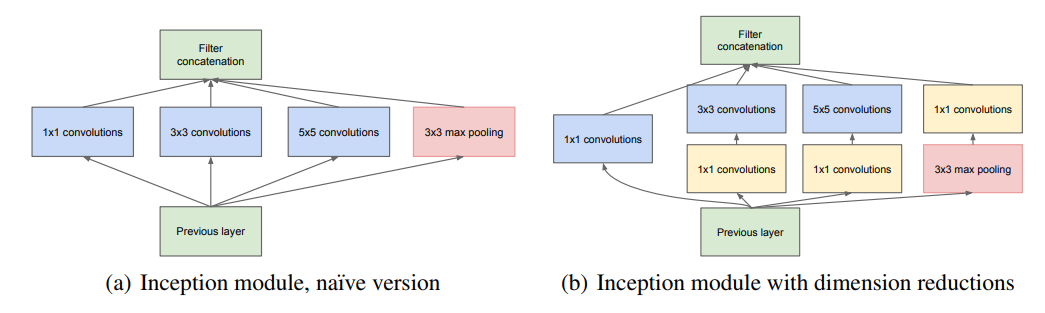
\includegraphics[width=14cm]{8_appendix/img/Inception_module.png}
      \caption{Inception Module \cite{szegedy2015going}.}
    \end{figure}
    Inception moduleは,小さな畳み込みフィルタを並列に並べることで,より少ないパラメータで同等の表現力を実現することが可能である.
    Inception moduleには1*1の畳み込みフィルタが使われているが,このフィルターは次元削減と等価な効果がある.
    \begin{figure}[ht]
      \centering
      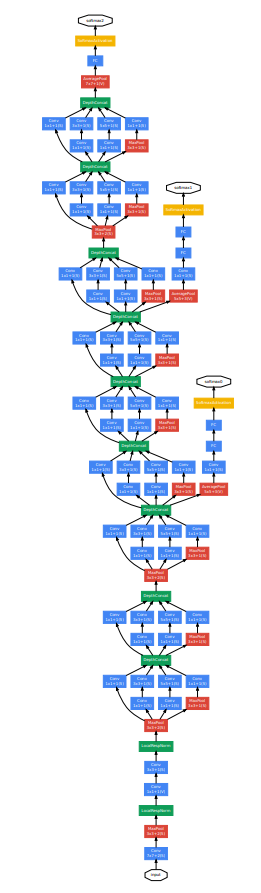
\includegraphics[width=4cm, angle=-90]{8_appendix/img/googlenet.png}
      \caption{Architecture of GoogLeNet \cite{szegedy2015going}.}
    \end{figure}
    
    GoogLeNetのもう一つの特徴として,補助的損失(auxiliary loss)がある.
    GoogLeNetはネットワークの途中から分岐させたサブネットワークにおいてクラス分類を行うような構造を持っており,これによってネットワークの中間層に直接誤差を伝播させ,勾配消失を抑える狙いがある.
    また,複数の損失関数があることにより,アンサンブル学習と同様の効果が得られるため,汎化性能の向上が期待できる.
    ここで,予測時は最終層の出力結果だけを用いることに注意されたい.
    
    このGoogLeNetはその構造の名前を取って一般にinceptionと呼ばれ,構造によってv1からv3まで細かい派生が存在する.
    GoogLeNetはこのv1に該当し,inception v2およびv3はGoogLeNetの畳み込み方法を変更し,モデルを更に多層化したものである.
    前節の畳み込み層の項で述べたが,カーネルサイズ3以上の畳み込みはカーネルサイズ3の畳み込みを複数適用することにより再現できる.
    そこで,v2では図\ref{convFactorization}のようにInception Moduleが改良されている.
    加えて,v2ではバッチ正規化が各層に導入されている.
    \begin{figure}[ht]
      \centering
      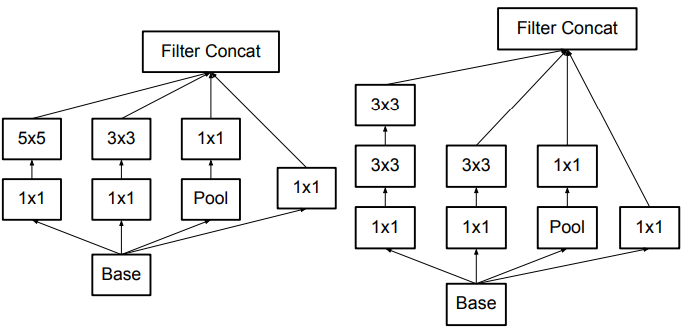
\includegraphics[width=12cm]{8_appendix/img/convFactorization}
      \caption{Factorization of Convolution.The left side is the original Inception Module and the right side is improved for v2 and v3.}
      \label{convFactorization}
    \end{figure}
    
    v3における重要な変更点は,畳み込みの素因数分解である.
    v3では以下の図\ref{improvements_inception}のような$n\times n$畳み込みを$n\times1$畳み込みと$1\times n$畳み込みに分割するモジュールが導入されている.
    これにより,単純な畳込みと比べて計算量が1/3減少する.
    他にも,効率的なグリッドサイズ削減モジュールも導入された.
    これは,従来プーリング層のみで行われていたグリッドサイズ削減を,ストライド2の畳み込みと組み合わせて行うことによって,より安価で効率的なネットワークが実現された.
    \begin{figure}[ht]
      \centering
      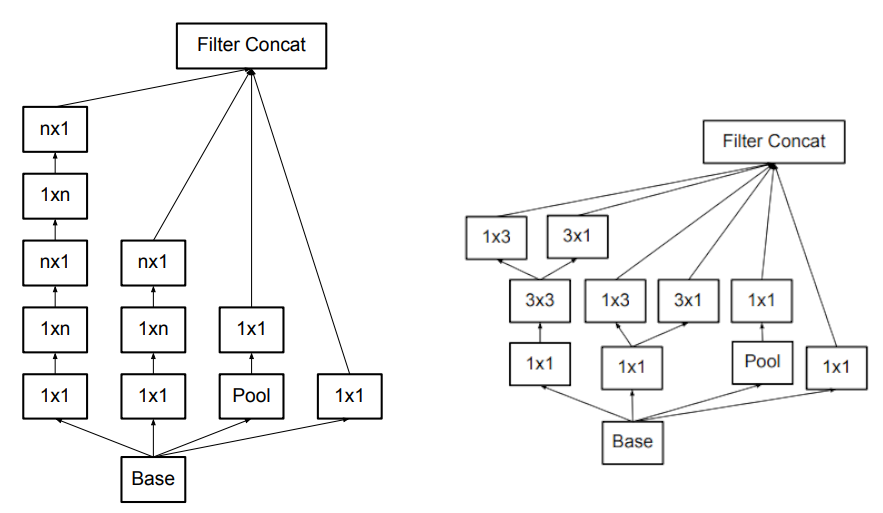
\includegraphics[width=12cm]{8_appendix/img/improvements_inception}
      \caption{Various improvements to the Inception Module.}
      \label{improvements_inception}
    \end{figure}

\subsubsection{ResNet}
    GoogLeNetでは補助的損失を用いて勾配消失を防いでいたが,補助的損失は構造が複雑になる上に,モデルのパラメータが増大するなど,様々な課題があった.
    ResNet\cite{he2016deep}ではResidual Block (残差ブロック)を導入することで,100層以上の深い構造であっても学習が可能となった.
    残差ブロックの概要図を図\ref{fig:residual_block}に示した.
    \begin{figure}[ht]
      \centering
      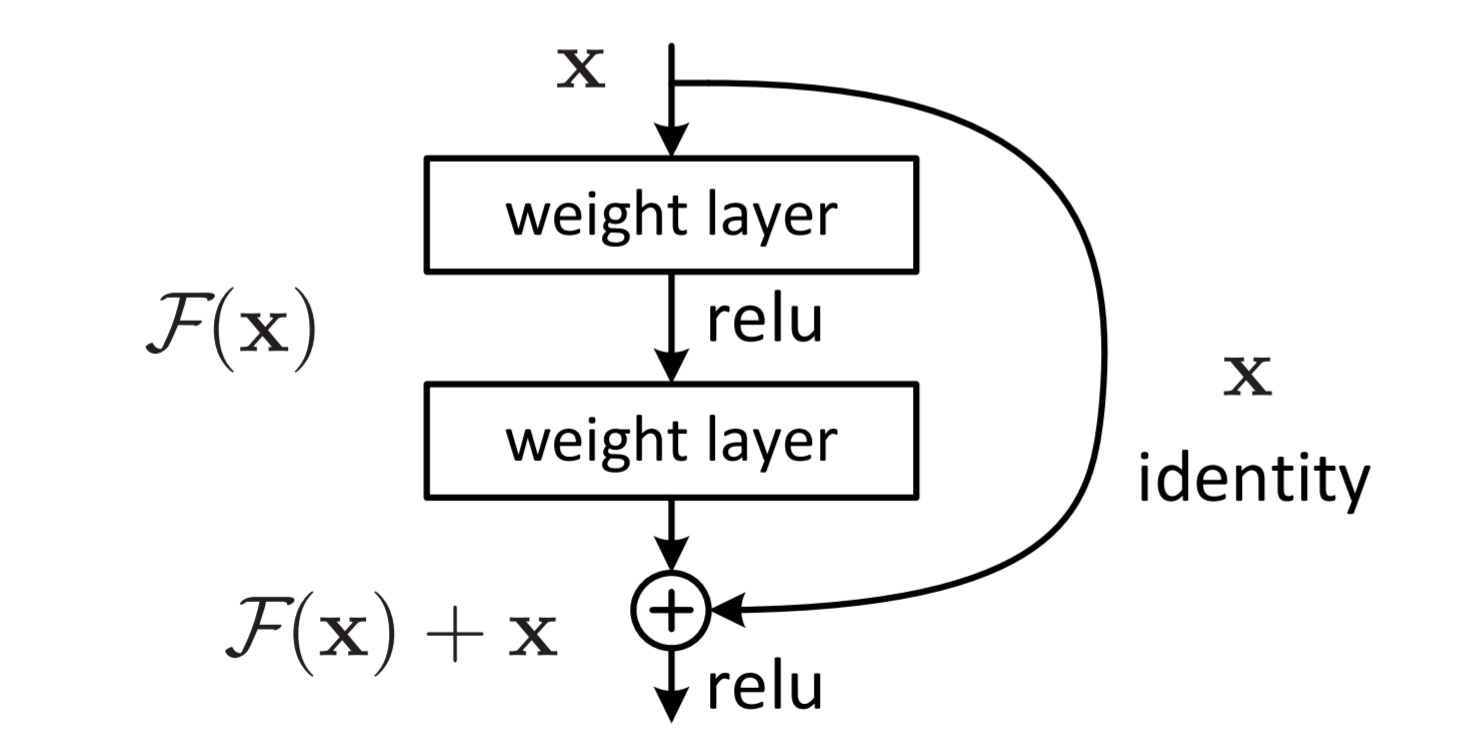
\includegraphics[width=10cm]{8_appendix/img/residual_block.png}
      \caption{Architecture of residual block \cite{he2016deep}.}
      \label{fig:residual_block}
    \end{figure}

    図のように,残差ブロックでは,入力されたデータが二つの経路に分かれる.
    一つが通常の畳み込み演算が行われる経路であり,もう一つが入力データをそのまま出力する経路(ショートカット接続)である.
    このショートカット接続が導入されたモデルの重要な特徴は3つ指摘されている.
    1つは,層をまたがる結合(Identity mapping)によって見かけのネットワークの深さが浅くなり,逆伝播計算時に勾配が減衰していくことを抑える効果をもたらした点である.
    
    そしてもう1つは,ショートカット接続により目的の出力を得るための学習から,残差の学習へと変化させることで,ネットワークが解きやすい問題に帰着させたことである.
    これによって,層が浅い場合でもモデルの高精度化を実現できるようになった.

    たとえば,層の途中で理想の特徴量が得られている場合,畳込みによって,入力と同じ出力を生成する必要があった.
    1つのピクセルに注目すると、各カーネルの各要素との積の総和が入力値と同様になるようなカーネルの重みを学習する必要がある.
    このようなカーネルの重みを学習するのは非常に困難である.
    しかし,残差を学習する場合には,畳込み層は負の値を出力するだけで活性化層で出力は0に是正され,残差ブロックの出力はショートカット接続により加算された入力値となる.
    
    最後は,層を過剰に深くした場合,過学習が発生するようになった点である.
    論文では,過剰に深いモデルを作成し,1202層のモデルでも学習が可能であり,精度が110層のモデル以下となったことを確認している.
    
     現在は,残差ブロックを導入したResNetを元に,様々な改良を施したネットワークの提案がなされている.
     Zagoruykoら\cite{zagoruyko2016wide}は各残差ブロックで増加する畳み込みのフィルタ数を大きくすることで,通常のResNetよりも浅いネットワークで優れた性能を有するを提案した.
     Hanら\cite{han2017deep}は残差ブロック間で急激にフィルタ数を大きくすることで,そのブロックの影響が他と比べて大きくなり,アンサンブル学習としての効果が薄れていると指摘し,各残差ブロックで徐々に畳み込みのフィルタ数を増加するようなネットワークを提案した.

\subsubsection{DenseNet}
    DenseNet\cite{huang2017densely}は,ResNetに似たショートカット結合をもつネットワークであり,その構造をDenseBlockと呼ぶ.
    DenseNetは,ResNet同様にショートカット結合を行っているため,勾配消失が起きにくい.
    ここで,ResNetと同様にショートカット接続を持っているが,足し合わせではなく,特徴量を結合していることの注意されたい.
    また,この構造により層の深さを抑えることができることによりパラメータ数を抑えることに成功している.
    
    \begin{figure}[ht]
      \centering
      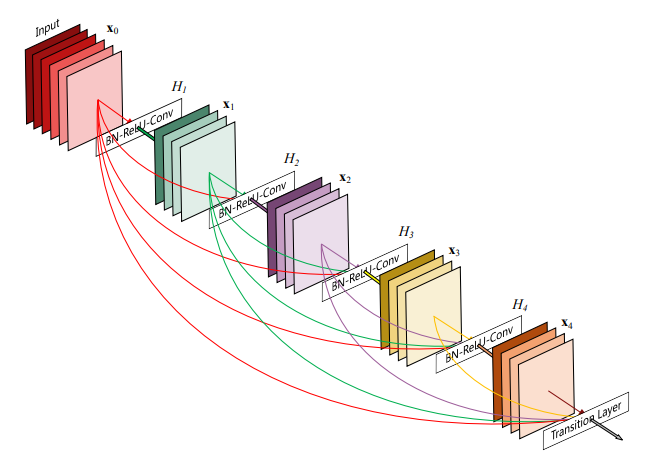
\includegraphics[width=10cm]{8_appendix/img/denseblock}
      \caption{Architecture of dense block \cite{huang2017densely}.}
      \label{fig:huang2017densely}
    \end{figure}
    
    チャンネル数kは成長率(Growth rate)と呼ばれ,ハイパーパラメータになる.
    また,図中のBN-ReLU-Convにおいて,異なる色の線はチャンネル方向に結合される.

\subsubsection{MobileNet}
    MobileNet\cite{howard2017mobilenets}はモバイル端末に乗せることのできる軽量かつ高性能なモデルを目標として設計されたCNNである。
    畳み込み層でDepthwise Separable Convolutionを用いることによって通常の畳み込みの1/9ほどに計算量を削減している。
    
    MobileNetは現在に至るまで複数の改良が施されている。
    MobileNet-v2\cite{sandler2018mobilenetv2}ではResNetで使われるResidual Blockを応用したInverted Residualを導入している。
    Residual Blockの計算量の多さを、Depthwise convolutionの前後にPointwise convolutionを挿入する構造を用いて解決している。
    
    MobileNet-v3\cite{howard2019searching}では、Squeeze-and-Exciteモジュールの導入によって、Self-Attentionを行うことによる精度向上を図っている。
    Depthwise convolutionはチャンネルごとに畳み込みを行うため、認識対象に特化した学習が可能になる。

\subsubsection{EfficientNet}
    EfficientNet\cite{tan2019efficientnet}は,モデルの深さ,広さ,解像度(入力画像の大きさ)の3つを調整することによりアーキテクチャにおける最適なモデルスケールアップを実現し,精度向上を達成したモデルである.
    EfficientNetはImageNetを含む5つのデータセットで当時の最高精度を達成した上に,従来のモデルよりもパラメータ数が非常に少ない.
    このモデルは構造が単純であり,転移学習でも効果を発揮する.
    
    EfficientNetはCompound Coefficient(複合係数) 導入し,この比率に従ってモデルの深さ,広さ,解像度の3つを調整されるMBConv\cite{howard2019searching}を多層化することによって構成されている.
    MBConvはMoble Inverted BottleneckにSEモジュールを追加したものであり、MobileNet-v3に採用されている構造である。
    その比率は以下のようになっている.
    \begin{eqnarray}
        \rm{depth:}d &=& \alpha^\phi \\
        \rm{width:}w &=& \beta^\phi \\
        \rm{resolution:}r &=& \gamma^\phi \\
        \rm{s.t.}\ \alpha&\cdot&\beta^{2}\cdot\gamma^{2}\approx2\\
        \alpha &\geq& 1, \beta \geq 1, \gamma \geq 1
    \end{eqnarray}
